\documentclass[11pt]{article}
\usepackage[margin=1in]{geometry}
\usepackage[T1]{fontenc}
\usepackage[utf8]{inputenc}
\usepackage{lmodern}
\usepackage{microtype}
\usepackage{amsmath,amssymb,bm}
\usepackage{xcolor}
\usepackage{booktabs}
\usepackage{hyperref}
\usepackage{enumitem}
\usepackage{fancyhdr}
\usepackage{tikz}
\usetikzlibrary{arrows.meta,calc,intersections,angles,quotes,positioning}

\hypersetup{colorlinks=true,linkcolor=blue!50!black,urlcolor=blue!50!black,citecolor=blue!50!black}
\pagestyle{fancy}
\fancyhf{}
\lhead{Dihedral Angle from a Three-Pentagon Patch}
\rhead{\thepage}
\setlength{\headheight}{14pt}

\definecolor{accent}{RGB}{31,73,125}
\definecolor{accent2}{RGB}{188,53,53}
\definecolor{softblue}{RGB}{224,236,248}
\definecolor{softgold}{RGB}{255,243,214}
\definecolor{softred}{RGB}{252,232,232}
\definecolor{softgray}{RGB}{243,245,247}

\newcommand{\cA}{\cos 36^\circ}
\newcommand{\sA}{\sin 36^\circ}
\newcommand{\cB}{\cos 72^\circ}
\newcommand{\sB}{\sin 72^\circ}
\newcommand{\R}{1}

\begin{document}

\begin{center}
    {\LARGE\bfseries An Educational Derivation of the Dodecahedron Dihedral Angle}\\[0.5em]
    {\large Folding a three-pentagon patch until two vertices coincide}\\[1em]
\end{center}

\noindent
\fcolorbox{accent!35}{softblue}{%
\begin{minipage}{0.965\linewidth}
\textbf{Main result.} If two congruent pentagon faces are folded out of the original \(xy\)-plane by the same physical angle and the moving vertices \(C\) and \(K\) are required to meet, then the fold angle is
\[
\boxed{\theta = \arccos\!\left(\frac{1}{\sqrt{5}}\right)=\arctan(2)\approx 63.43494882^\circ.}
\]
The corresponding \emph{internal dihedral angle} of the regular dodecahedron is
\[
\boxed{\delta = 180^\circ-\theta \approx 116.56505118^\circ.}
\]
\end{minipage}}

\vspace{1em}

\begin{abstract}
This note shows how a local patch of three regular pentagons already contains the dihedral angle of the regular dodecahedron. We first set up a coordinate model, then derive the exact fold angle using Rodrigues' rotation formula and a symmetry condition. We also give a numerical minimization viewpoint, which is often the most practical way to solve related folding problems computationally.
\end{abstract}

\section*{1. Geometric setup}
At the shared vertex \(O\), the relevant directions in the planar pentagon patch are the hinge edges \(OA\) and \(OH\), together with the moving edges \(OC\) and \(OK\). We place \(O\) at the origin and normalize lengths so that \(|OA|=|OH|=|OC|=|OK|=1\).

A convenient choice of coordinates is
\[
A=(-\cos 36^\circ,\; \sin 36^\circ,\; 0),
\qquad
H=(\cos 36^\circ,\; \sin 36^\circ,\; 0),
\]
\[
C=(-\cos 72^\circ,\; -\sin 72^\circ,\; 0),
\qquad
K=(\cos 72^\circ,\; -\sin 72^\circ,\; 0).
\]

\begin{figure}[h!]
\centering
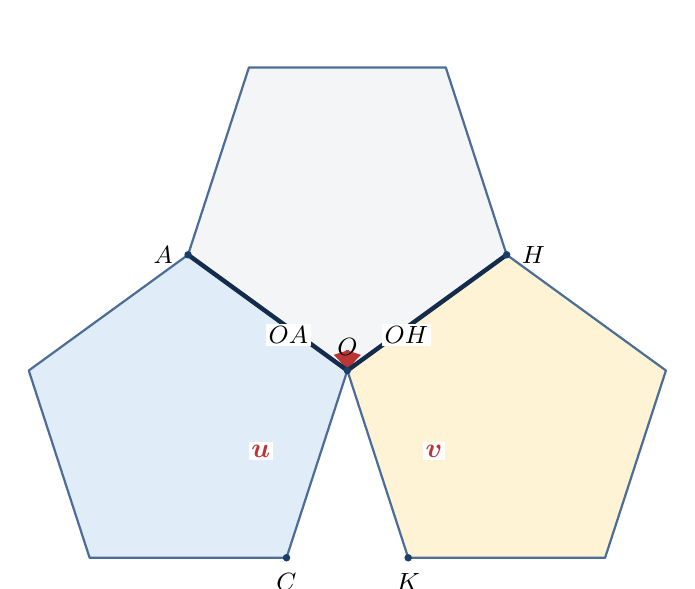
\begin{tikzpicture}[scale=2.5, line join=round, line cap=round, >=Latex]
    % exact planar three-pentagon patch with unit edge length
    \coordinate (O) at (0,0);
    \coordinate (A) at (-0.80901699,0.58778525);
    \coordinate (F) at (-0.50000000,1.53884177);
    \coordinate (G) at ( 0.50000000,1.53884177);
    \coordinate (H) at ( 0.80901699,0.58778525);
    \coordinate (C) at (-0.30901699,-0.95105652);
    \coordinate (D) at (-1.30901699,-0.95105652);
    \coordinate (E) at (-1.61803399, 0.00000000);
    \coordinate (K) at ( 0.30901699,-0.95105652);
    \coordinate (J) at ( 1.30901699,-0.95105652);
    \coordinate (I) at ( 1.61803399, 0.00000000);

    % fills use the same cyclic order as the outlines
    \fill[softblue] (O)--(C)--(D)--(E)--(A)--cycle;
    \fill[softgray] (O)--(A)--(F)--(G)--(H)--cycle;
    \fill[softgold] (O)--(H)--(I)--(J)--(K)--cycle;

    % outlines
    \draw[thick,accent!80] (O)--(C)--(D)--(E)--(A)--cycle;
    \draw[thick,accent!80] (O)--(A)--(F)--(G)--(H)--cycle;
    \draw[thick,accent!80] (O)--(H)--(I)--(J)--(K)--cycle;

    % key vectors
    \draw[very thick,accent2,-{Latex[length=2.8mm]}] (O)--($(C)!0.985!(O)$);
    \draw[very thick,accent2,-{Latex[length=2.8mm]}] (O)--($(K)!0.985!(O)$);
    \node[accent2,fill=white,inner sep=1pt] at (-0.44,-0.41) {$\bm u$};
    \node[accent2,fill=white,inner sep=1pt] at ( 0.44,-0.41) {$\bm v$};

    % hinge edges
    \draw[ultra thick,accent!60!black] (O)--(A);
    \draw[ultra thick,accent!60!black] (O)--(H);

    % only the essential labels
    \foreach \P in {O,A,C,H,K} {\fill[accent!85!black] (\P) circle (0.019);}
    \node[font=\small,above=2pt] at (O) {$O$};
    \node[font=\small,left=2pt] at (A) {$A$};
    \node[font=\small,below=2pt] at (C) {$C$};
    \node[font=\small,right=2pt] at (H) {$H$};
    \node[font=\small,below=2pt] at (K) {$K$};
    \node[font=\small,fill=white,inner sep=1pt] at (-0.30,0.18) {$OA$};
    \node[font=\small,fill=white,inner sep=1pt] at ( 0.30,0.18) {$OH$};
\end{tikzpicture}
\caption{The planar three-pentagon patch. The center face stays in the original plane, and the two side faces fold about the hinge edges \(OA\) and \(OH\). Only the moving vertices \(C\) and \(K\) are labeled.}
\end{figure}

\paragraph{What folds, exactly?}
The left face is rotated out of the plane about the axis \(OA\). The right face is rotated by the same \emph{physical} fold angle about the axis \(OH\). In a right-hand-rule convention these two rotations carry opposite signs, so we write
\[
C_\theta = R_{OA}(\theta)\,C,
\qquad
K_\theta = R_{OH}(-\theta)\,K.
\]
Because the configuration is mirror-symmetric about the plane \(x=0\), the meeting point must lie in that symmetry plane.

\section*{2. Exact derivation}
Let
\[
a = \overrightarrow{OA} = (-\cos 36^\circ,\; \sin 36^\circ,\; 0),
\qquad
c = \overrightarrow{OC} = (-\cos 72^\circ,\; -\sin 72^\circ,\; 0).
\]
The Rodrigues formula for rotating a vector \(c\) about the unit axis \(a\) is
\[
R_a(\theta)c = c\cos\theta + (a\times c)\sin\theta + a\,(a\cdot c)(1-\cos\theta).
\]
We only need the \(x\)-coordinate of \(C_\theta=R_a(\theta)c\).

Two quick computations are enough:
\[
a\cdot c = \cos 36^\circ\cos 72^\circ - \sin 36^\circ\sin 72^\circ
=\cos 108^\circ = -\cos 72^\circ,
\]
and since \(a\) and \(c\) lie in the \(xy\)-plane,
\[
a\times c = (0,0,\sin 72^\circ).
\]
Therefore the cross-product term contributes no \(x\)-component, and
\begin{align*}
 x(C_\theta)
 &= -\cos 72^\circ\cos\theta + (-\cos 36^\circ)(-\cos 72^\circ)(1-\cos\theta)\\[0.3em]
 &= \cos 72^\circ\cos 36^\circ - \cos 72^\circ(1+\cos 36^\circ)\cos\theta.
\end{align*}
Now use the exact identities
\[
\cos 72^\circ\cos 36^\circ = \frac14,
\qquad
\cos 72^\circ\bigl(1+\cos 36^\circ\bigr)=\frac{\sqrt5}{4}.
\]
This gives the compact formula
\[
\boxed{x(C_\theta)=\frac{1-\sqrt5\cos\theta}{4}.}
\]

By symmetry \(K_\theta\) is the mirror image of \(C_\theta\) across the plane \(x=0\). Hence \(C_\theta\) and \(K_\theta\) meet if and only if \(x(C_\theta)=0\). So
\[
\frac{1-\sqrt5\cos\theta}{4}=0
\qquad\Longrightarrow\qquad
\cos\theta=\frac1{\sqrt5}.
\]
Thus
\[
\boxed{\theta = \arccos\!\left(\frac{1}{\sqrt5}\right)=\arctan(2)\approx 63.43494882^\circ.}
\]

\begin{figure}[h!]
\centering
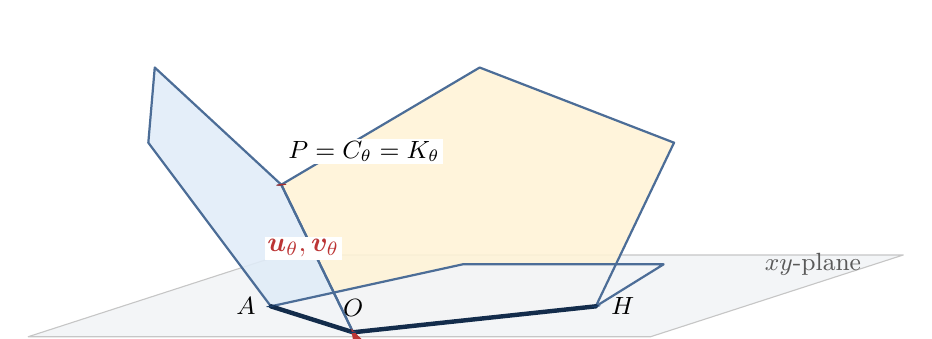
\begin{tikzpicture}[scale=2.55, x={(1cm,0cm)}, y={(0.68cm,0.22cm)}, z={(0cm,1cm)}, line join=round, line cap=round, >=Latex]
    % central face in the xy-plane
    \coordinate (O) at (0,0,0);
    \coordinate (A) at (-0.80901699,0.58778525,0);
    \coordinate (F) at (-0.50000000,1.53884177,0);
    \coordinate (G) at ( 0.50000000,1.53884177,0);
    \coordinate (H) at ( 0.80901699,0.58778525,0);

    % folded side faces at the meeting angle
    \coordinate (P) at ( 0.00000000,-0.52573111,0.85065081);
    \coordinate (D) at (-0.80901699,-0.26286556,1.37638192);
    \coordinate (E) at (-1.30901699, 0.42532540,0.85065081);
    \coordinate (J) at ( 0.80901699,-0.26286556,1.37638192);
    \coordinate (I) at ( 1.30901699, 0.42532540,0.85065081);

    % faint reference plane
    \fill[softgray] (-1.55,-0.10,0) -- (1.55,-0.10,0) -- (1.55,1.75,0) -- (-1.55,1.75,0) -- cycle;
    \draw[gray!45] (-1.55,-0.10,0) -- (1.55,-0.10,0) -- (1.55,1.75,0) -- (-1.55,1.75,0) -- cycle;
    \node[gray!70!black,font=\small] at (1.25,1.53,0) {$xy$-plane};

    % faces, back to front
    \fill[softblue,fill opacity=0.88] (O)--(P)--(D)--(E)--(A)--cycle;
    \fill[softgold,fill opacity=0.88] (O)--(H)--(I)--(J)--(P)--cycle;
    \fill[softgray,fill opacity=0.96] (O)--(A)--(F)--(G)--(H)--cycle;

    \draw[thick,accent!80] (O)--(P)--(D)--(E)--(A)--cycle;
    \draw[thick,accent!80] (O)--(H)--(I)--(J)--(P)--cycle;
    \draw[thick,accent!80] (O)--(A)--(F)--(G)--(H)--cycle;

    % hinge axes and folded vectors
    \draw[ultra thick,accent!60!black] (O)--(A);
    \draw[ultra thick,accent!60!black] (O)--(H);
    \draw[very thick,accent2,-{Latex[length=2.6mm]}] (O)--($(P)!0.97!(O)$);
    \draw[very thick,accent2,-{Latex[length=2.6mm]}] (O)--($(P)!0.97!(O)$);

    % essential labels only
    \foreach \Q in {O,A,H,P} {\fill[accent!85!black] (\Q) circle (0.020);}
    \node[font=\small,above=2pt] at (O) {$O$};
    \node[font=\small,left=2pt] at (A) {$A$};
    \node[font=\small,right=2pt] at (H) {$H$};
    \fill[accent2!90!black] (P) circle (0.022);
    \node[font=\small,fill=white,inner sep=1pt] at (0.30,-0.36,0.98) {$P=C_{\theta}=K_{\theta}$};
    \node[accent2,fill=white,inner sep=1pt] at (-0.18,-0.10,0.44) {$\bm u_{\theta},\bm v_{\theta}$};
\end{tikzpicture}
\caption{A cleaner 3D view at the meeting angle. The center face stays in the \(xy\)-plane while the two side faces rotate about \(OA\) and \(OH\) until the moving vertices coincide at \(P\).}
\end{figure}

\section*{3. A numerical solution by error minimization}
The same answer can be recovered without symbolic manipulation. Define the squared mismatch
\[
E(\theta)=\|C_\theta-K_\theta\|^2.
\]
This is a nonnegative scalar function of a single variable. The physically correct fold angle is the minimizer of \(E\); at the true meeting angle the mismatch is exactly zero.

For the present geometry,
\[
E(\theta)=\bigl\|R_{OA}(\theta)C-R_{OH}(-\theta)K\bigr\|^2,
\]
and a one-dimensional search over \(0^\circ\le \theta\le 90^\circ\) gives a unique minimum at
\[
\theta\approx 63.43495^\circ.
\]

\begin{figure}[h!]
\centering
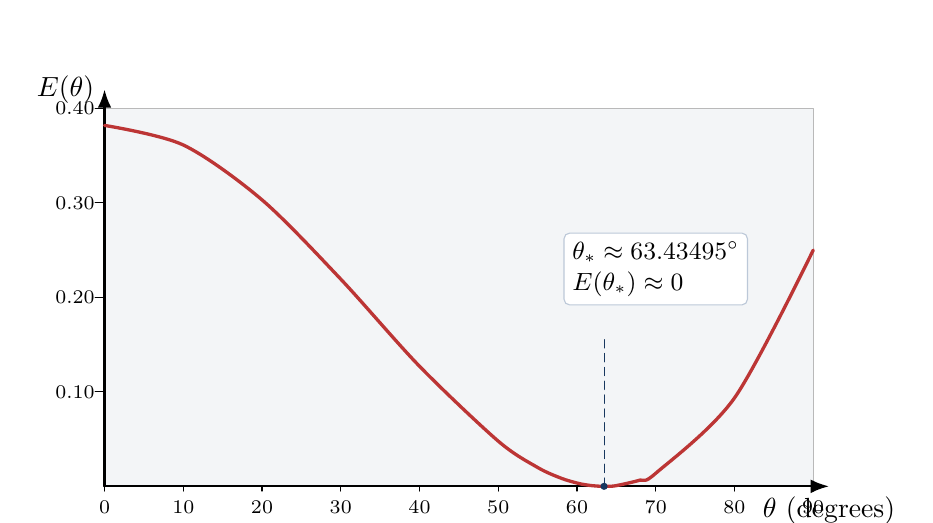
\begin{tikzpicture}[x=0.10cm,y=12cm, line join=round, line cap=round, >=Latex]
    % frame
    \fill[softgray] (0,0) rectangle (90,0.40);
    \draw[gray!55] (0,0) rectangle (90,0.40);
    % axes
    \draw[->,thick] (0,0) -- (92,0) node[below] {$\theta$ (degrees)};
    \draw[->,thick] (0,0) -- (0,0.42) node[left] {$E(\theta)$};
    % ticks
    \foreach \x in {0,10,20,30,40,50,60,70,80,90} {
        \draw (\x,0) -- (\x,-0.005) node[below,font=\scriptsize] {\x};
    }
    \foreach \y/\lab in {0.10/0.10,0.20/0.20,0.30/0.30,0.40/0.40} {
        \draw (-1.2,\y) -- (0,\y) node[left,font=\scriptsize] {\lab};
    }
    % curve
    \draw[very thick,accent2]
        plot[smooth] coordinates {
            (0.00000,0.381966)
            (10.00000,0.361259)
            (20.00000,0.303169)
            (30.00000,0.219254)
            (40.00000,0.127066)
            (50.00000,0.047811)
            (55.00000,0.019959)
            (58.00000,0.008550)
            (60.00000,0.003483)
            (61.00000,0.001767)
            (62.00000,0.000619)
            (63.00000,0.000057)
            (63.43495,0.000000)
            (64.00000,0.000098)
            (65.00000,0.000756)
            (68.00000,0.006590)
            (70.00000,0.013832)
            (80.00000,0.093548)
            (90.00000,0.250000)
        };
    % minimum marker
    \draw[accent!75!black,densely dashed] (63.43495,0) -- (63.43495,0.16);
    \fill[accent!75!black] (63.43495,0) circle (1.3pt);
    \node[fill=white,draw=accent!30,rounded corners=2pt,inner sep=3pt,align=left,font=\small] at (70,0.23)
    {$\theta_*\approx 63.43495^\circ$\\$E(\theta_*)\approx 0$};
\end{tikzpicture}
\caption{Squared mismatch between the two moving vertices. The minimizer occurs exactly where the two points meet.}
\end{figure}

\paragraph{Why this numerical viewpoint matters.}
The minimization formulation generalizes immediately to more complicated nets, non-regular faces, or situations where an exact symbolic derivation is inconvenient. In practice one can use a simple grid search followed by Brent's method or Newton refinement.

\section*{4. From fold angle to dihedral angle}
The fold angle \(\theta\) is the amount each face is rotated out of the original plane. The \emph{internal dihedral angle} \(\delta\) of the regular dodecahedron is the supplement of that fold angle:
\[
\boxed{\delta = 180^\circ - \theta.}
\]
Substituting the value above gives
\[
\boxed{\delta = 180^\circ - \arctan(2) \approx 116.56505118^\circ.}
\]
This is the familiar exact angle for a regular dodecahedron.

\vspace{0.7em}
\noindent
\fcolorbox{accent!35}{softgold}{%
\begin{minipage}{0.965\linewidth}
\textbf{Takeaway.} The entire dihedral-angle calculation boils down to a local matching condition in a three-pentagon patch. Symmetry reduces the geometry to one scalar equation, and the same geometry also appears naturally as a one-variable minimization problem.
\end{minipage}}

\end{document}
